\input ../SlidePreamble
\input ../preamble

\begin{document}

{\Huge

  \centerline{\bf TTIC 31230, Fundamentals of Deep Learning}
  \bigskip
  \centerline{David McAllester, Winter 2018}
  \vfill
  \centerline{\bf Loopy Graphical Models}
\vfill
\vfill
\vfill
\slide{The Big Picture I}

Conditional vs. Unconditional

\vfill
$$\Phi^* = \argmin_\Phi E_{(x,y) \sim \mathrm{Pop}}\;-\ln \;P(y|x)$$

\vfill
$$\Phi^* = \argmin_\Phi E_{y \sim \mathrm{Pop}}\;-\ln \;P(y)$$

\vfill
This is a non-distinction: the issues in the to the conditional case
are exactly the same as in the unconditional case.

\slide{The Big Picture II}

The structured case: $y \in {\cal Y}$ where ${\cal Y}$ is discrete but iteration over $\hat{y} \in {\cal Y}$ is infeasible.

\vfill
{\color{red} Graphical models rely on assumptions about the structure of $P_\Phi(y)$.}

\vfill
{\color{red} Loopy Graphical Models can use weaker assumptions than those supporting exact computation of $P_\Phi(y)$.}

\vfill
{\color{red} For loopy graphical Models there are various methods of performing approximate gradient descent on cross-entropy loss.}

\slide{Colorization --- a Self-Supervised Problem}

\centerline{\includegraphics[height = 2in]{../images/colorization}}

$x$ is a black and white image.

\vfill
$y$ is a ``color'' image drawn from $\pop(y|x)$ where the color has been rounded to one of, say, 100 color words.

\vfill
$\hat{y}$ is an arbitrary color image.

\vfill
$P_\Phi(\hat{y}|x)$ is the probability that model $\Phi$ assigns to the color image $\hat{y}$ given black and white image $x$.

\slide{Colorizing Superpixels}
\centerline{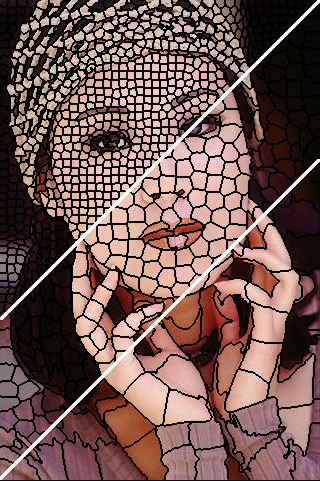
\includegraphics[height = 3in]{../images/SLIC} \hspace{.5in} 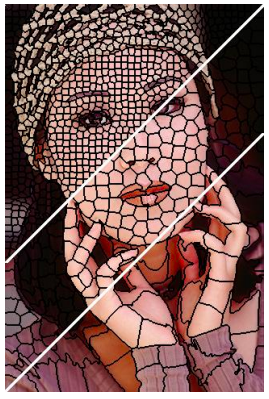
\includegraphics[height = 3in]{../images/SLICcolor}}
\centerline{\huge SLIC superpixels, Achanta et al.}

\vfill
$\hat{y}[i]$ is the color value of superpixel $i$ in color image $\hat{y}$.

\vfill
$\hat{y}[(i,j)]$ is the pair $(\hat{y}[i],\hat{y}[j])$ for neighbors $i$ and $j$.

\slide{Exponential Softmax}

\begin{eqnarray*}
P_\Phi(\hat{y}|x) & = & \softmax_{\hat{y}}\;s_\Phi(\hat{y}|x)
\end{eqnarray*}

\vfill
Let ${\cal C}$ be colors, ${\cal I}$ be superpixels, and ${\cal E}$ be edges.

\vfill
We will compute

\vfill {\bf a unary potential tensor} $s_i[c] = s_\Phi(c|x,i)$

\vfill
{\bf a binary potential tensor} $s_e[c,c'] = s_\Phi(c,c'|x,e)$

\vfill
$$s_\Phi(\hat{y}|x) = \sum_{i \in {\cal I}} s_i[\hat{y}[i]] + \sum_{e \in {\cal E}}\;s_e[\hat{y}[e.i],\hat{y}[e.j]]$$

\slide{Backpropagation}

The input is the image $x$ and the parameter package $\Phi$

\begin{eqnarray*}
 & \vdots & \\
s_i[c] & = & \ldots \\
s_e[c,c'] & = & \ldots \\
{\cal L} & = & - \ln\; P(y\;|\;s_{\cal I}[{\cal C}],\;s_{\cal E}[{\cal C}, {\cal C}])
\end{eqnarray*}

\vfill
We need to compute $s_i.\grad[c]$ and $s_e.\grad[c,c']$.

\slide{General Markov Random Fields (MRFs)}

\centerline{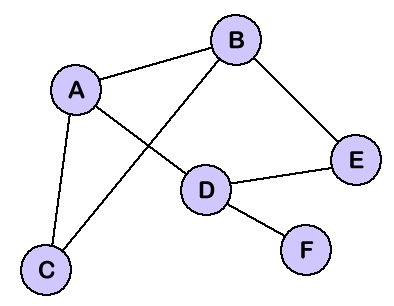
\includegraphics[height= 1.5in]{../images/Graph}}

$$s(\hat{y}) = \sum_{i \in \mathrm{Nodes}}\; s_i[\hat{y}[i]]\; + \sum_{e \in \mathrm{Edges}}\;s_e[\hat{y}[e.i],\hat{y}[e.j]]$$

\vfill
\centerline{Node Potentials \hspace{4em}Edge Potentials}

\slide{An Example}

Consider an image with three superpixels $A$, $B$ and $C$ where
each superpixel is to labeled as either ``foreground'' or background.

\vfill
Suppose the unary potentials are all zero.

\vfill
$$s_A(\mathrm{Foreground}) = s_A(\mathrm{Background}) = 0$$
$$s_B(\mathrm{Foreground}) = s_B(\mathrm{Background}) = 0$$
$$s_C(\mathrm{Foreground}) = s_C(\mathrm{Background}) = 0$$

\slide{The Binary Potentials}


\vfill
Let $F_A$ be the proposition that $A$ is forground and similarly for $F_B$ and $F_C$.

\vfill
We can express $P_A \Rightarrow P_B$ with
$$s_{A,B}(\mathrm{Foreground},\mathrm{Background}) = -1$$
$$s_{A,B}(\mathrm{Foreground},\mathrm{Foreground}) = 1$$
$$s_{A,B}(\mathrm{Background},\mathrm{Background}) = 1$$
$$s_{A,B}(\mathrm{Background},\mathrm{Foreground}) = 1$$

\vfill
The binary potentials are then given by
$F_A \Rightarrow F_B$, $F_B \Rightarrow F_C$, $F_C \Rightarrow F_A$.

\slide{The Full Configuration Potential}

For any configuration $\hat{y}$ we have that $s(\hat{y})$ is the sum of the unary and binary potentials.

\vfill
If none are foreground we have $s(\hat{y}) = 3$

\vfill
If one is foreground we have $s(\hat{y}) = -1 + 1+ 1 = 1$

\vfill
If two are foreground we also have $s(\hat{y}) = -1 + 1+ 1 = 1$

\vfill
If all are foreground we have $s(\hat{y}) = 3$.

\vfill
$$Z = 6*1 + 2*3 = 12\;\;\;\;P_A(\mathrm{Foregound}) = \frac{3*1 + 3}{12} = \frac{1}{2}$$

\slide{Hyper-Graphs: More General and More Concise}

A hyper-edge is a subset of nodes.

\vfill
\centerline{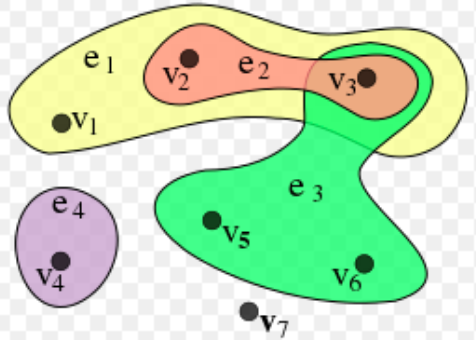
\includegraphics[height = 1.5in]{../images/HyperGraph}}


$$s(\hat{y}) = \sum_{i \in \mathrm{Nodes}}\; s_i[\hat{y}[i]]\; + \sum_{e \in \mathrm{Edges}}\;s_e[\hat{y}[e.i],\hat{y}[e.j]]$$

\vfill

$${\color{red} s(\hat{y}) = \sum_{e \in \mathrm{HyperEdges}}  \; s_e[\hat{y}[e]]}$$


\slide{Backpropagation}

The input is the image $x$ and the parameter package $\Phi$

\begin{eqnarray*}
 & \vdots & \\
s_e[\hat{y}] & = & \ldots \\
{\cal L} & = & - \ln\; P(y\;|\;s_{\cal E}[{\cal Y}])
\end{eqnarray*}

\vfill We abbreviate $P(\hat{y}\;|\;s_{\cal E}[{\cal Y}])$ as {\color{red} $P_s(\hat{y})$} --- the distribution on $\hat{y}$ defined by the tensor $s$.
\vfill
We need to compute {\color{red} $\nabla_s -\ln P_s(y)$}, or equivalently, {\color{red} $s_e.\grad[\tilde{y}]$}.

\ignore{
\slidetwo{Generative Fully Observed Models}
{(Language Models) are Tractable}

\centerline{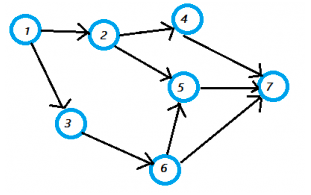
\includegraphics[height=1.5in]{../images/DAG} \hspace{1in} 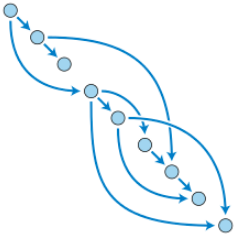
\includegraphics[height=1.5in]{../images/SortedDAG}}

\vfill
An auto-regressive model is locally normalized.

\begin{eqnarray*}
  P_s(\hat{y}) & = & \prod_i \; P_s(\hat{y}[i]\;|\; \hat{y}[\mathrm{Parents}(i)]) \\
  \\
  P_s(\hat{y}[i]\;|\; \hat{y}[\mathrm{Parents}(i)])  & = &  \softmax_{\tilde{y}} s(\tilde{y}|\hat{y}[\mathrm{Parents}(i)])
\end{eqnarray*}

\vfill
There are exponentially many possible values for $\hat{y}$ but each softmax is over a tractable-sized set.
}

\slideplain{Back-Propagation Through An Exponential Softmax}

\bigskip
\begin{eqnarray*}
  \mathrm{loss}(s,y) & = & - \ln \left(\frac{1}{Z(s)}\;e^{s(y)}\right) \\
  \\
  & = & \ln Z(s) - s(y) \\
  \\
  \\
  s_e.\mathrm{grad}[\tilde{y}]
    & = & \left(\frac{1}{Z} \sum_{\hat{y}} e^{s(\hat{y})} \left(\partial s(\hat{y})/\partial s_e[\tilde{y}]\right)\right)
    - \left(\partial s(y) /\partial s_e[\tilde{y}]\right)
\end{eqnarray*}

\slide{Back-Propagation Through An Exponential Softmax}

\bigskip
\begin{eqnarray*}
    s_e.\mathrm{grad}[\tilde{y}]
    & = & \left(\frac{1}{Z} \sum_{\hat{y}} e^{s(\hat{y})} \left(\partial s(\hat{y})/\partial s_e[\tilde{y}]\right)\right)
    - \left(\partial s(y) /\partial s_e[\tilde{y}]\right)    \\
    \\
    & = & \left(\sum_{\hat{y}} P_s(\hat{y}) \left(\partial s(\hat{y})/\partial s_e[\tilde{y}]\right)\right)
    - \left(\partial s(y) /\partial s_e[\tilde{y}]\right)    \\
    \\
    & = & E_{\hat{y} \sim P_s}\bbone[\hat{y}[e] = \tilde{y}]
    - \mathbbm{1}[y[e] = \tilde{y}] \\
    \\
    & = & {\color{red} P_{\hat{y} \sim P_s}(\hat{y}[e] = \tilde{y})}
      - \mathbbm{1}[y[e] = \tilde{y}]
\end{eqnarray*}

\slide{Hyperedge Marginals}

\begin{eqnarray*}
    s.\mathrm{grad}[e,\tilde{y}]
    & = &  {\color{red} P_{\hat{y} \sim P_s}(\hat{y}[e] = \tilde{y})} - \bbone[y[e] = \tilde{y}] \\
\end{eqnarray*}

\vfill
We will write {\color{red} $P_e(\tilde{y})$} for {\color{red} $P_{\hat{y} \sim P_s}(\hat{y}(e) = \tilde{y})$}.

\vfill
To compute $s.\mathrm{grad}$ it suffices to compute ${\color{red} P_e(\tilde{y})}$.

\vfill
We now focus on computing the hyperedge marginals for a given hyperedge score function (MRF) $s$.

\ignore{
\slide{An Aside: Features and Weights}

The indicators $\mathbbm{1}[\hat{y}[e] = \tilde{y}]$ form a 0-1 feature vector $\Psi(\hat{y})$.

\vfill
The tensor $s[e,\;\tilde{y}]$ forms a weight vector.

\begin{eqnarray*}
s(\hat{y}) & = & \sum_e s[e,\hat{y}[e]] \\
\\
& = & \sum_{e,\tilde{y}}\;s[e,\tilde{y}] \mathbbm{1}[e, \hat{y}[e] = \tilde{y}] \\
\\
& = & f^\top \Psi(\hat{y})
\end{eqnarray*}

\slide{An Aside: Features and Weights}

The hyperedge marginals  ${\color{red} P_{\hat{y} \sim P_s}(\hat{y}[e] = \tilde{y})}$ are just the expected value of the features under the distribution
defined by the MRF.
}

\slidetwo{For Tree-Strutured Models}{The Hyperedge Marginals Can be Computed Exactly}

\begin{eqnarray*}
  s.\mathrm{grad}[e,\tilde{y}] & = & {\color{red} P_e(\tilde{y})} - \mathbbm{1}[y[e] = \tilde{y}]
\end{eqnarray*}

\vfill
\centerline{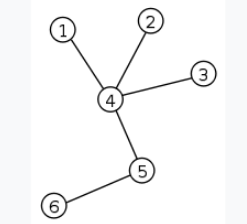
\includegraphics[height= 2in]{../images/Tree}}

\vfill
For trees we can compute $P_{e}(\tilde{y})$ exactly by message passing, a.k.a., belief propagation.

\anaslide{Defining the Messages}

\centerline{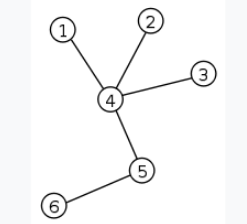
\includegraphics[height=1.5in]{../images/Tree}}

\vfill
For each edge $\{i,j\}$ and possible value $\tilde{y}$ for node $i$ we define {\color{red} $Z_{j \rightarrow i}[\tilde{y}]$}
to be  the partition function for the subtree attached to $i$ through $j$ and
with $\hat{y}[i]$ restricted to $\tilde{y}$.

\vfill
The function $Z_{j \rightarrow i}$ on the possible values of node $i$ is called the {\bf message} from $j$ to $i$.

\vfill
The reverse direction message $Z_{i \rightarrow j}$ is defined similarly.

\slide{Computing the Messages}

\centerline{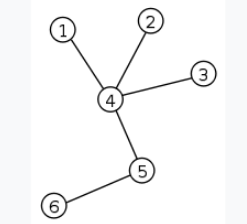
\includegraphics[height=2.0in]{../images/Tree}}

\vfill
\begin{eqnarray*}
  Z_{j\rightarrow i}[\tilde{y}] & = & \sum_{\tilde{y}'}  e^{s_j[\tilde{y}'] + s_{\{j,i\}}[\{\tilde{y}',\tilde{y}\}]}
    \left(\prod_{k \in N(j),\;k \not = i}\;Z_{k\rightarrow j}[\tilde{y}']\right)
\end{eqnarray*}

\anaslide{Computing Node Marginals from Messages}

\centerline{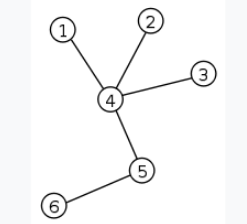
\includegraphics[height=1.5in]{../images/Tree}}

\begin{eqnarray*}
Z_i(\tilde{y}) & \doteq & \sum_{\hat{y}:\; \hat{y}[i] = \tilde{y}} \;e^{s(\hat{y})} \\
\\
& = & e^{s_i[\tilde{y}]} \left(\prod_{j\in N(i)} Z_{j \rightarrow i}[\tilde{y}]\right) \\
\\
{\color{red} P_i(\tilde{y})} & = & Z_i(\tilde{y})/Z,\;\;\;\;\; Z = \sum_{\tilde{y}}\;Z_i(\tilde{y})
\end{eqnarray*}


\anaslide{Computing Edge Marginals from Messages}

\begin{eqnarray*}
Z_{\{i,j\}}(\tilde{y}) & \doteq & \sum_{\hat{y}:\; \hat{y}[\{i,j\}] = \tilde{y}} \;e^{s(\hat{y})} \\
\\
& = & e^{s[i,\tilde{y}[i]] + s[j,\tilde{y}[j]] +s[\{i,j\},\tilde{y}]} \\
& & \prod_{k\in N(i),\;k \not = j} Z_{k \rightarrow i}[\tilde{y}[i]] \\
& & \prod_{k\in N(j),\;k \not = i} Z_{k \rightarrow j}[\tilde{y}[j]] \\
\\
{\color{red} P_{\{i,j\}}(\tilde{y})} & = & Z_{\{i,j\}}(\tilde{y})/Z
\end{eqnarray*}

\slide{Loopy BP}

Message passing is also called belief propagation (BP).

\vfill
In a graph with cycles it is common to do {\bf Loopy BP}.

\vfill
This is done by initializing all message $Z_{i \rightarrow j}[\tilde{y}] = 1$ and then repeating (until convergence) the updates
\vfill
\begin{eqnarray*}
  P_{j \rightarrow i}[\tilde{y}] & = & \frac{1}{Z}\;Z_{j \rightarrow i}[\tilde{y}] \;\;\;\;\;Z = \sum_{\tilde{y}} Z_{j \rightarrow i}[\tilde{y}] \\
  \\
  \\
  Z_{j\rightarrow i}[\tilde{y}] & = & \sum_{\tilde{y}'}  e^{s[j,\tilde{y}'] + s[\{j,i\},\{\tilde{y}',\tilde{y}\}]}
    \left(\prod_{k \in N(j),\;k \not = i}\;P_{k\rightarrow j}[\tilde{y}']\right)
\end{eqnarray*}

\slide{Other Methods of Approximating Hyperedge Marginals}

MCMC Sampling

\vfill
Constrastive Divergence

\vfill
Pseudo-Liklihood

\slide{The Big Picture I}

Conditional vs. Unconditional

\vfill
$$\Phi^* = \argmin_\Phi E_{(x,y) \sim \mathrm{Pop}}\;-\ln \;P(y|x)$$

\vfill
$$\Phi^* = \argmin_\Phi E_{y \sim \mathrm{Pop}}\;-\ln \;P(y)$$

\vfill
This is a non-distinction: the issues in the to the conditional case
are exactly the same as in the unconditional case.

\slide{The Big Picture II}

The number of possible values of $y$.

\vfill
The binary case: $y \in \{-1,1\}$.

\vfill
The multiclass case: $y \in {\cal Y}$ where iteration over $\hat{y} \in {\cal Y}$ is feasible.

\vfill
{\color{red} The structured case: $y \in {\cal Y}$ where ${\cal Y}$ is discrete but iteration over $\hat{y} \in {\cal Y}$ is infeasible.}

\slide{The Big Picture I}

Conditional vs. Unconditional

\vfill
$$\Phi^* = \argmin_\Phi E_{(x,y) \sim \mathrm{Pop}}\;-\ln \;P(y|x)$$

\vfill
$$\Phi^* = \argmin_\Phi E_{y \sim \mathrm{Pop}}\;-\ln \;P(y)$$

\vfill
This is a non-distinction: the issues in the to the conditional case
are exactly the same as in the unconditional case.

\slide{The Big Picture II}

The structured case: $y \in {\cal Y}$ where ${\cal Y}$ is discrete but iteration over $\hat{y} \in {\cal Y}$ is infeasible.

\vfill
{\color{red} Graphical models rely on assumptions about the structure of $P_\Phi(y)$.}

\vfill
{\color{red} Loopy Graphical Models can use weaker assumptions than those supporting exact computation of $P_\Phi(y)$.}

\vfill
{\color{red} For loopy graphical Models there are various methods of performing approximate gradient descent on cross-entropy loss.}
\slide{END}

}
\end{document}

